\documentclass[12pt,a4paper]{article} 

\usepackage{fn2kursstyle}
\usepackage[russian]{babel}
\usepackage[T2A]{fontenc} 
\usepackage[utf8]{inputenc} 
\usepackage{geometry}
\usepackage{mathtools}
\usepackage{tikz}
\usepackage{chngcntr}

\counterwithout{equation}{section}
\frenchspacing 

\title{Модель двух конкурирующих видов}
\group{ФН2-42Б}
\author{А.\,И.~Токарев}
\supervisor{М.\,П.~Галанин}
\date{2021}

\newcommand*\circled[1]{\tikz[baseline=(char.base)]{
            \node[shape=circle,draw,inner sep=2pt] (char) {#1};}}

\makeatletter
\newenvironment{sqcases}{%
  \matrix@check\sqcases\env@sqcases
}{%
  \endarray\right.%
}
\def\env@sqcases{%
  \let\@ifnextchar\new@ifnextchar
  \left\lbrack
  \def\arraystretch{1.2}%
  \array{@{}l@{\quad}l@{}}%
}
\makeatother

\begin{document}
    \maketitle
    \tableofcontents
    \pagebreak

    \section-{Введение}
    \pagebreak

    \section{Постановка задачи}
    Рассмотрим некоторые задачи из области динамики популяций. Пусть есть два сходных вида, конкурирующих между собой за пищу. Очевидно, что возможны следующие варианты: 
    \begin{itemize}
        \item Выживает только первый вид;
        \item Выживает только второй вид;
        \item Выживают оба вида;
        \item Оба вида вымирают.
    \end{itemize}
    
    Каждый из этих вариантов соответствует наличию своего положения равновесия. Тем самым для описания данной системы нужна модель с четырьмя неподвижными точками --- стационарными состояниями системы.

    В соответствии с гипотезой В.\,Волтера\footnote{В.\,Волтера (\textit{ит.} Vito Volterra, 1860--1940) --- итальянский математик и физик.} модель двух конкурирующих видов выглядит следующим образом:
    \begin{equation}
        \label{volterra}
        \begin{cases}
            \frac{dx_1}{dt} = a_1 x_1 - b_{12} x_1 x_2 - c_1 {x_1}\!^2,
            \\
            \frac{dx_2}{dt} = a_2 x_2 - b_{21} x_2 x_1 - c_2 {x_2}\!^2 ,
        \end{cases}
    \end{equation}
    \noindent где $a_1, a_2$ --- коэфициенты скорости роста популяции; $b_{12}, b_{21}$ --- коэфициенты межвидовой борьбы; $c_1, c_2$ --- внутривидовой борьбы первого и второго вида соответсвенно.

    В данной курсовой работе необходимо рассмотреть все варианты параметров системы и исследовать качественное поведение ее решений. Также важно уделить внимание особым точкам системы.

    \section{Стационарные состояния}

    Найдем стационарные точки. Для этого необходимо решить СЛАУ вида: 
    \begin{equation}
        \label{stationarySLAE}
        \begin{cases}
            a_1 x_1 - b_{12} x_1 x_2 - c_1 {x_1}\!^2 = 0,
            \\
            a_2 x_2 - b_{21} x_2 x_1 - c_2 {x_2}\!^2 = 0,
        \end{cases}
    \end{equation}
    \pagebreak
    
    \noindent откуда получаем 4 стационарных состояния:
    \begin{enumerate}
        \setlength\itemsep{0.5em}
        \item $ x_1 = 0,\ x_2 = 0 $ --- вымирание обоих видов;
        \item $ x_1 = 0,\ x_2 = \dfrac{a_2}{c_2} $ --- вымирание первого вида, достижение вторым видом конечной численности $ \dfrac{a_2}{c_2} $;
        \item $ x_1 = \dfrac{a_1}{c_1},\ x_2 = 0 $ --- противоположная ситуация, то есть достижение первым видом численности $ \dfrac{a_1}{c_1} $ и вымирание второго вида;
        \item $ x_1 = \dfrac{a_1 c_2 - a_2 b_{12}}{c_1 c_2 - b_{12} b_{21}},\ x_2 = \dfrac{a_2 c_1 - a_1 b_{21}}{c_1 c_2 - b_{12} b_{21}}$ --- выживание обоих видов.
    \end{enumerate} 

    \vspace{1em}Особое внимание стоит уделить 4 стационарному состоянию. Решения $ x_1,\ x_2 $ в этой ситуации должны быть положительными. Условия положительности неподвижных решений выполняются в одном из двух случаях: 

    \begin{table}[h]
        \centering
        \begin{tabular}{rl}
            \circled{1}
            &
            $
                \begin{cases}
                    a_1 c_2 > a_2 b_{12},
                    \\
                    a_2 c_1 > a_1 b_{21},
                    \\
                    c_1 c_2 > b_{12} b_{21}
                \end{cases}
            $
            \\[15mm]
            \circled{2}
            &
            $
                \begin{cases}
                    a_1 c_2 < a_2 b_{12},
                    \\
                    a_2 c_1 < a_1 b_{21},
                    \\
                    c_1 c_2 < b_{12} b_{21}
                \end{cases}
            $
        \end{tabular}
    \end{table}

    Также расположение стационарных точек можно продемонстрировать на графике. Каждое из уравнений (\refeq{stationarySLAE}) задает прямую-сепаратрису:
    \begin{equation}
        \label{nullclines}
        \begin{sqcases}
            \begin{cases}
                x_1 = 0,
                \\
                x_2 = \dfrac{a_1 + c_1 x_1}{b_{12}},
            \end{cases}
            \\[1cm]
            \begin{cases}
                x_1 = 0,
                \\
                x_2 = \dfrac{a_1 + c_1 x_1}{b_{12}}
            \end{cases}
        \end{sqcases}
    \end{equation}
    
    Попарные пересечения сепаратрис дают стационарные состояния. Возможные взаимные расположения прямых-сепаратрис приведены на рис. 1:

    \begin{figure}[h!]
        \centering
        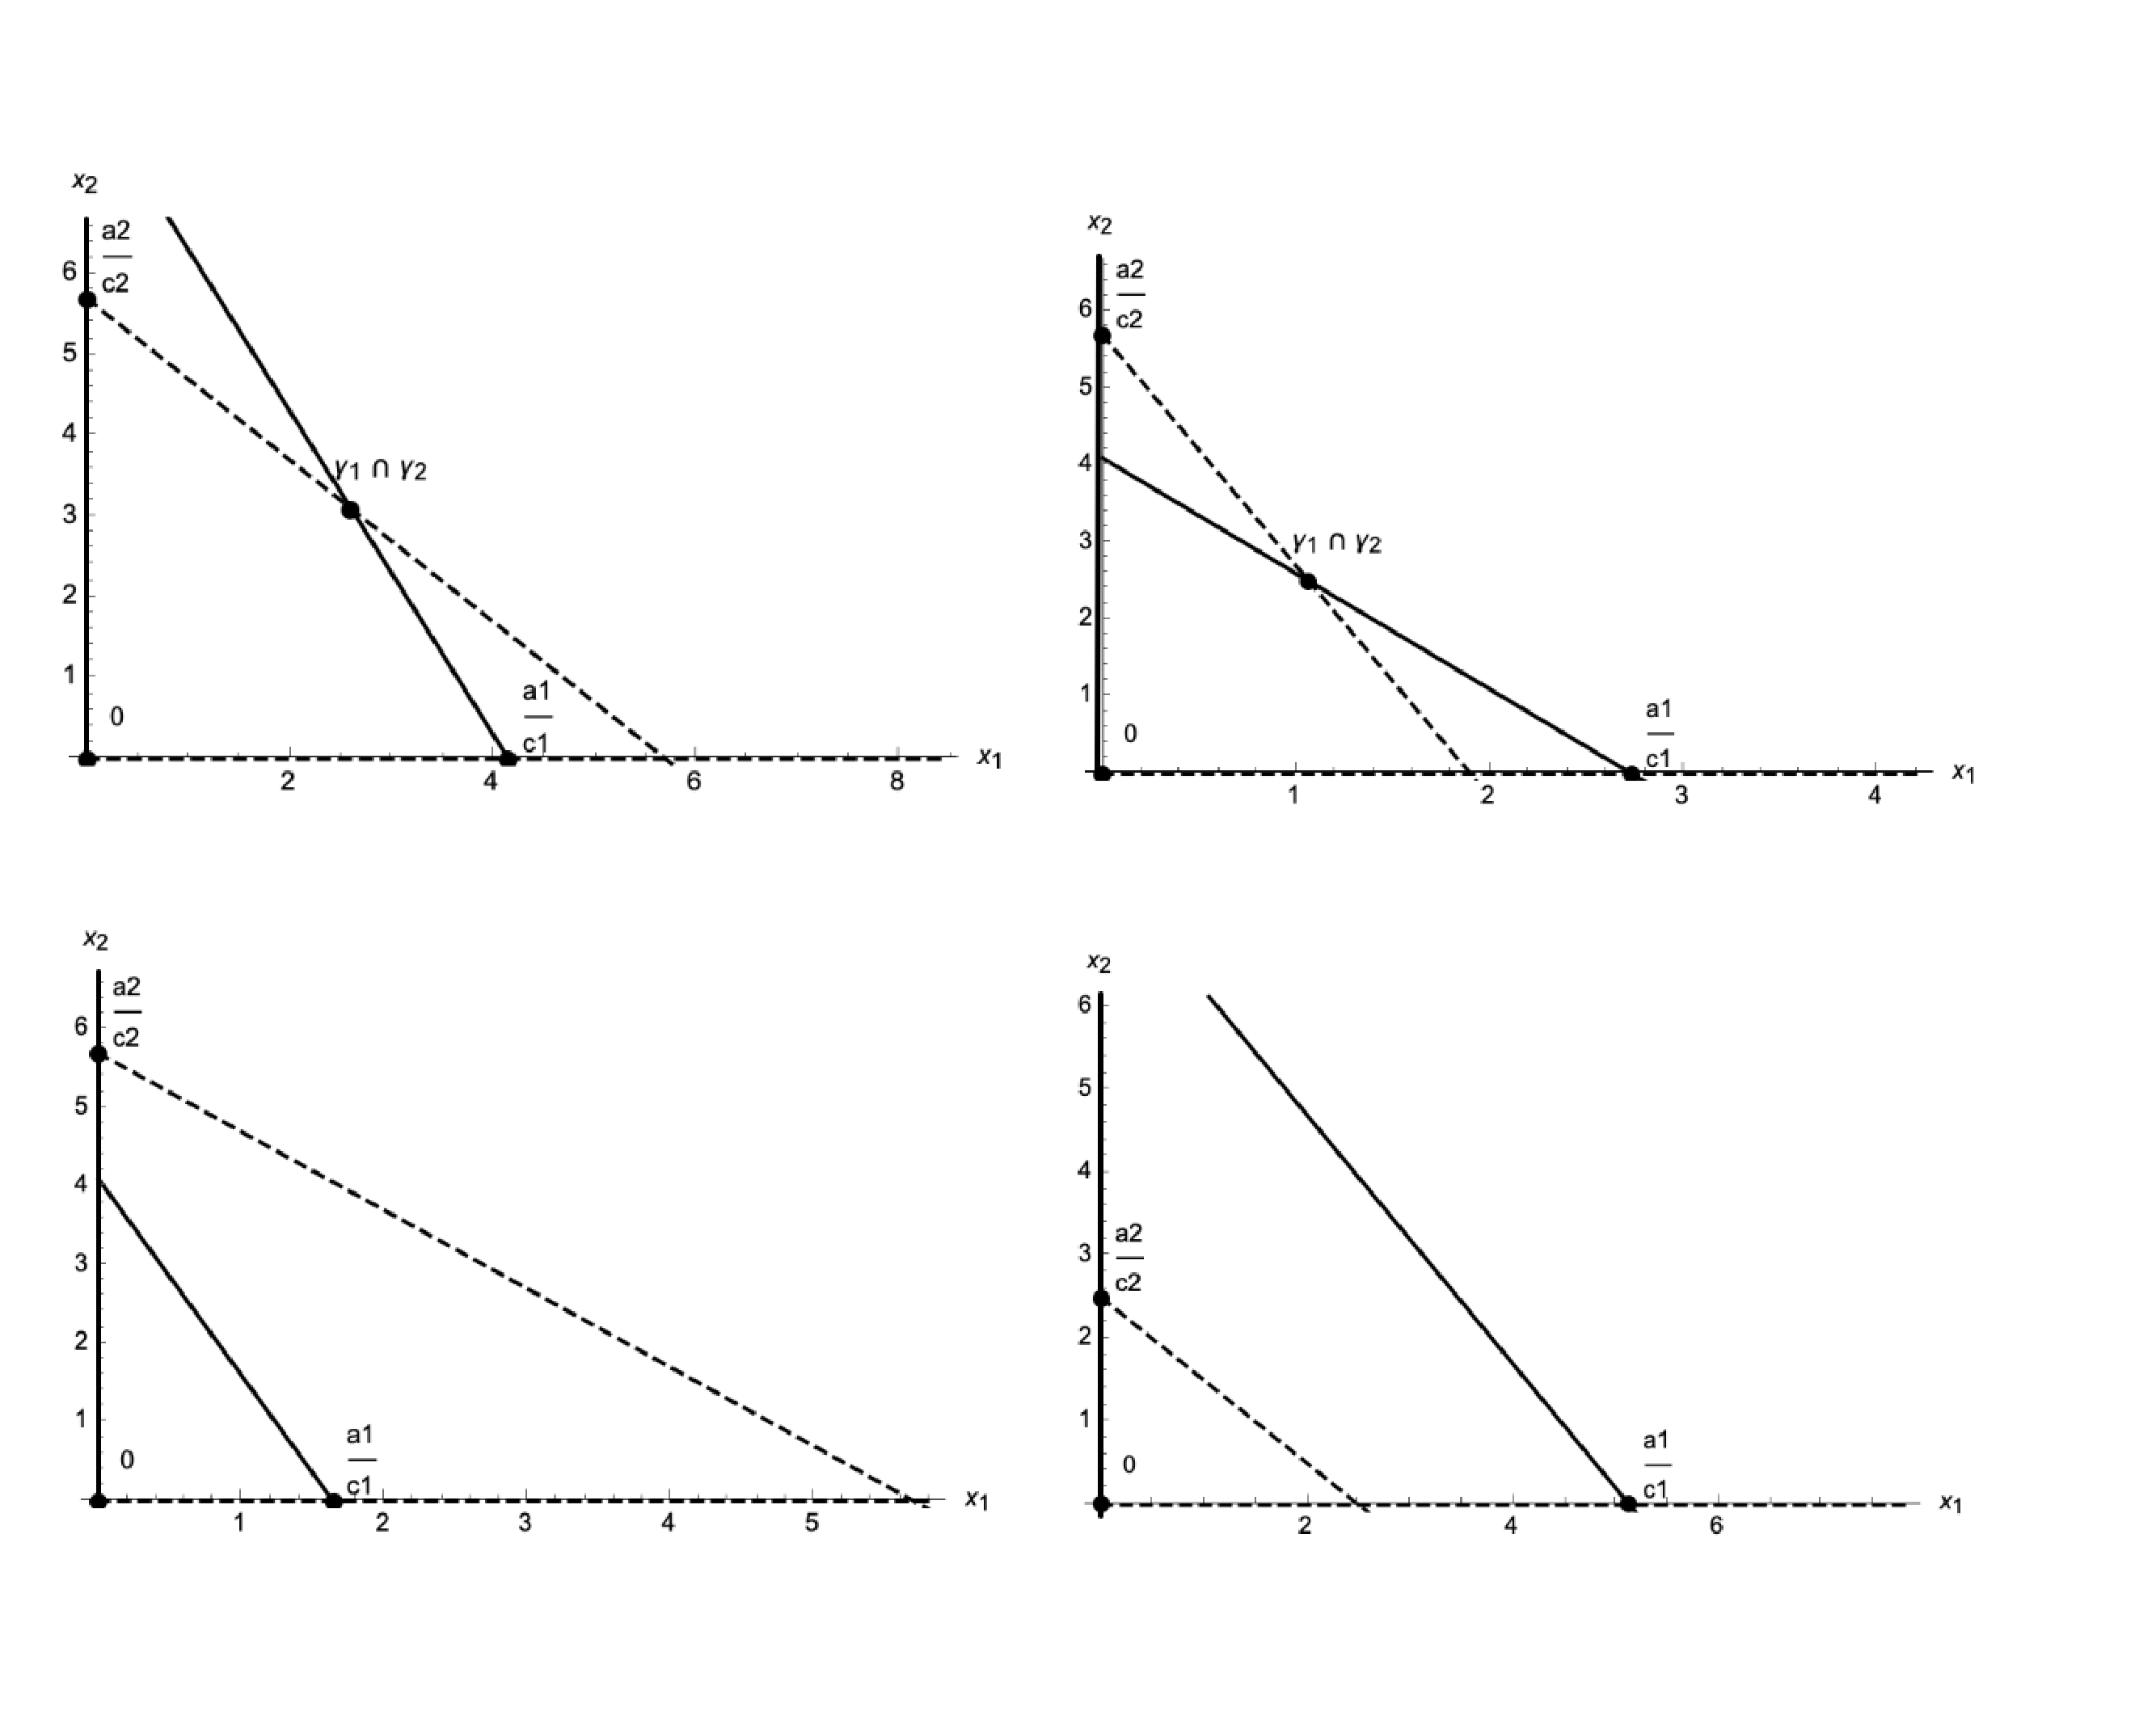
\includegraphics[width=\textwidth]{separatrises.pdf}
        \caption{Расположение сепаратрис системы в зависимости от параметров.}
        \label{fig:seps}
    \end{figure}

    Линеаризация системы --- построение приближенной линейной модели. Линеаризуем нашу систему: 
    \[
        \mathbb{J} = 
            \begin{pmatrix}
                a_1 - b_{12} x_2 - 2 c_1 x_1 & -b_{12} x_1
                \\
                -b_{21} x_2 & a_2 - b_{21} x_1 - 2c_2 x_2
            \end{pmatrix}
    \]

    \end{document}
